\documentclass[class=article]{standalone}
%----------------------------Preamble-------------------------------%
\usepackage{tikz}                       % Drawing/graphing tools.
\usetikzlibrary{positioning}            % Relative positioning of nodes.
%--------------------------Main Document----------------------------%
\begin{document}
    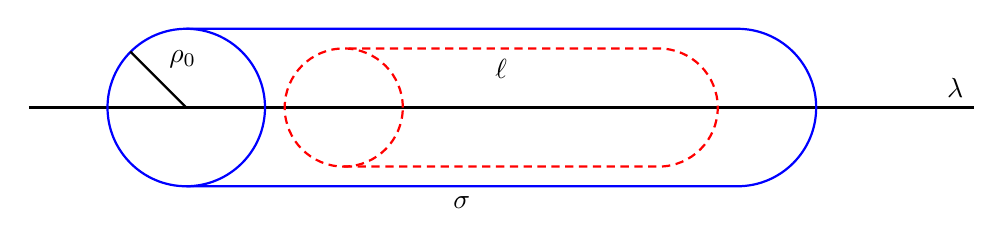
\begin{tikzpicture}[every path/.style={thick}]
        \draw (-6,0) -- (6,0) node[above left] {$\lambda$};
        \draw[draw=blue] (-4,0) circle (1);
        \draw[draw=blue] (-4,1) -- (3,1) arc (90:-90:1)
            to node[below] {$\sigma$} (-4,-1);
        \draw[draw=red,densely dashed]  (-2,0) circle (0.75);
        \draw (-4,0) to node[above right=0.02 and 0.01]
            {$\rho_{0}$} (-4.71,0.71);
        \draw[draw=red,densely dashed] (-2,-0.75) to (2,-0.75)
            arc (-90:90:0.75) to node[below] {$\ell$} (-2,0.75);
    \end{tikzpicture}
\end{document}